\documentclass{article} % For LaTeX2e
\usepackage{iclr2017_conference,times}
\usepackage[hidelinks]{hyperref}
\usepackage{url}

\usepackage{natbib}
\usepackage{graphicx}
\usepackage{floatrow}
\usepackage{appendix}
\usepackage{caption}
\captionsetup{compatibility=false}
\usepackage{subcaption}
\usepackage[justification=centering]{caption}

\title{Overcoming Partial Observability with Recurrent Neural Networks}


\author{Guillaume Berger \\
	\texttt{guillaume.berger@umontreal.ca}\\
}

% The \author macro works with any number of authors. There are two commands
% used to separate the names and addresses of multiple authors: \And and \AND.
%
% Using \And between authors leaves it to \LaTeX{} to determine where to break
% the lines. Using \AND forces a linebreak at that point. So, if \LaTeX{}
% puts 3 of 4 authors names on the first line, and the last on the second
% line, try using \AND instead of \And before the third author name.

\newcommand{\fix}{\marginpar{FIX}}
\newcommand{\new}{\marginpar{NEW}}

%\iclrfinalcopy % Uncomment for camera-ready version

\begin{document}
	
	\maketitle
	
	
	\begin{abstract}
		In reinforcement learning (RL) tasks, the environment is most of the time assumed to be Markovian : the optimal decision only depends on the current state. We say that the task is a Markovian Decision Process (MDP). Unfortunately, most real-world applications are not MDPs but Partialy Observable MDPs (POMDP) : knowing the current state is not sufficient to select the best action. POMDP are more challenging because the agent needs to be able to look back to past interactions in order to behave optimally. In other words, better performance will be achieved if the agent has a memory mechanism which allows him to overcome partial observability. Due to their hidden states which are persistent over time, recurrent neural networks (RNN) provide a way of storing memories of past interactions. In this work, we compare RNNs with other approaches such as feedforward Deep Q-Networks (DQN) [2] and Memory Networks [6] on a GridWorld example. Results illustrate the benefits of using RNNs in the context of partial observability.
	\end{abstract}
	
	
	\section{Introduction}
	
	
	\paragraph{The limit of feedforward DQNs:} Deep Q-Networks (DQNs) have recently known great successes, especially with Atari 2600 games, on which they achieved state-of-the-art results [2, 3]. A DQN agent is learning policies from raw pixels exploiting a CNN trained via Q-Learning. Although training such agents is hard, long, and requires some tricks (Experience Replay, usage of a target network...), obtained policies are above or near-human performance on many Atari games. However, DQNs are limited: they take decisions from a fixed number of past observations. More concretely, a DQN agent trained on an Atari game usually takes its decisions based on the last four observed frames (see Figure \ref{fig:a}).
		
	
	Due to its limited receptive field over past interactions, such agent would not be able to master tasks in which it is important to remember information from early timesteps. On Atari games, it does not really matter because knowing only the last 4 frames is sufficient to determine the optimal policy. In other words, for Atari games, including the last four observed frames in the state representation is enough to make the environment be Markovian. Nevertheless, we could easily imagine games, or real-word applications, where the ability to store memories of past interactions would be important to take good decisions. A DQN, as presented in Figure \ref{fig:a}, would not be well equipped for this kind of task.
	
	\paragraph{Partial Observability:} Unfortunately, in many real-world applications, the entire world is not visible at any moment, but partially observable. In this context, the environment does not meet the standards of a MDP because the current state is not sufficient to select the optimal policy: we say that the environment is a Partialy Observable Markov Decision Processes (POMDP). In order to master POMDPs, it is important to allow the agent to store (and read from) memories of past interactions. Deep Recurrent Q-Networks (DRQN) [1] provide a way of achieving this. Therefore, we expect that recurrent nets should overcome feedforward ones on POMDPs.
	
	\paragraph{Recurrent Neural Networks:} As illustrated in Figure \ref{fig:b}, designing the architecture of a DRQN could simply consist in adding one recurrent layer on top of feedforward ones. In comparison with feedforward layers, recurrent ones have hidden states that are persistent over time:

	$$ h_{t+1} = \Phi(U \ x_{t+1}  +  W \ h_t) $$
	
	where  $h_t$  represents the hidden states,  $x_{t+1}$  is the new input at timestep  $t+1$ , and  $\Phi$  is a non-linearity. Therefore, at timestep $T$, the hidden states  $h_T$ depends on all previously visited states  $h_t$, $t<T$. Consequently, one can hope that a DRQN agent would be able to exploit past experience thanks to its recurrent hidden states. Note that, in practice, one would probably prefer LSTM layers, for which the recurrent equation is more complex, over simple recurrent layers as they are better at learning long-term dependencies.
	
	In [1], they compared DQNs and DRQNs, trained on POMDP versions of Atari games. Results illustrate the benefit of incorporating recurrent layers in the architecture of the function approximator: as expected, DRQNs better handle partial observability. Inspired by [1], our work is aimed at reproducing these results on our own environment and comparing RNNs with other architecture such as Memory networks [6].
	
	\begin{figure}
		\begin{subfigure}[b]{.45\linewidth}
			\centering
			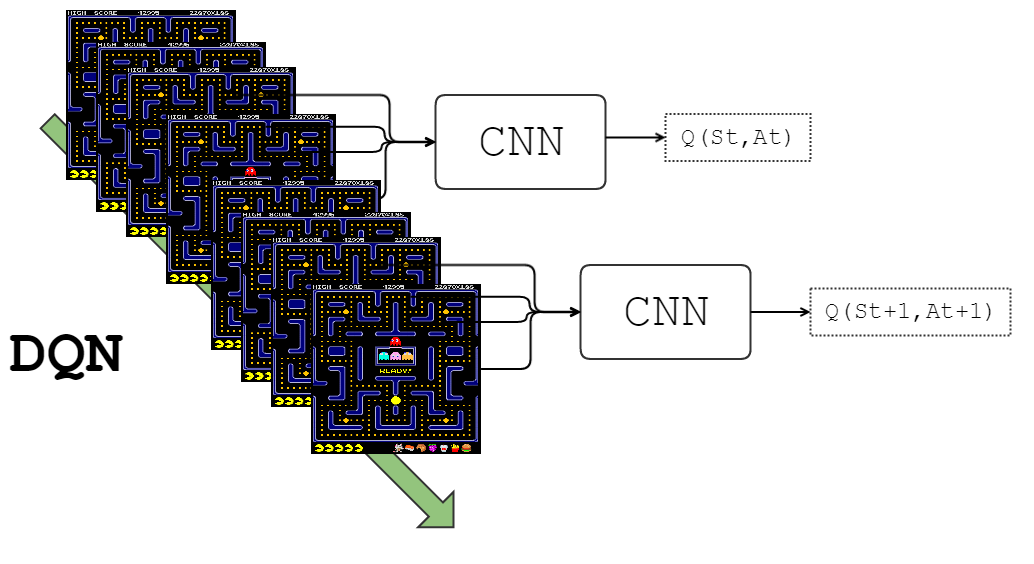
\includegraphics[height=3cm]{imgs/DQN.png}
			\caption{Feedforward DQN}
			\label{fig:a}
		\end{subfigure}
		\begin{subfigure}[b]{.45\linewidth}
			\centering
			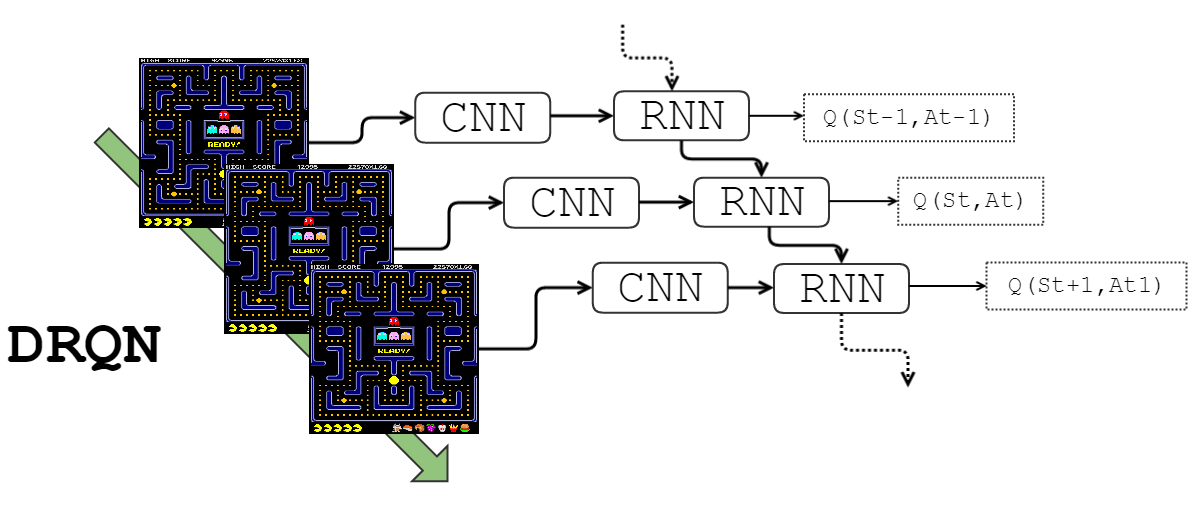
\includegraphics[height=3cm]{imgs/DRQN.png}
			\caption{Recurrent DQN}
			\label{fig:b}
		\end{subfigure}
		\caption{Two different neural net approaches for playing Atari.}\label{fig:1}
	\end{figure}
	
	
	
	\paragraph{Related work}: While giving the opportunity of storing memories to the agent is not a novel idea (e.g. [7]), this memory mechanism seems to be a hot topic currently:
	the very recent DeepMind paper [5] investigates a mechanism that allows the agent to store past experiences. However, their memory mechanism seems to be mostly aimed at speeding up the training of DQNs rather than improving performance on POMDPs.
	
	\section{Experiments}
	
	\paragraph{GridWorld rules :} Our environment is the $7 \times 7$ GridWorld represented in Figure \ref{grid}. The agent (blue cell) has 4 possible actions : \textit{left, right, up, down}. When the agent moves on a green cell, the reward is  $+0.5$. On the contrary, when the agent moves on a red cell, the reward is  $-1.0$. For any other move, the reward is  -0.1 . When a green cell or a red cell is reached, it re-appears elsewhere. This environment is taken from [8].
	
	\paragraph{Tricks:}
	
	It is well-known that training DQN via Q-learning is hard, and most of the time, we need to use few tricks to make it work. In our case, we used Experience Replay and a distinct Target Network whose weights are updated at the end of every episode.
	
	\paragraph{Some hyperparameter values:}
	
	For all the experiments reported below, we used the following hyperparemter values: 
	
	\begin{itemize}
		\item Discount factor: $\gamma = 0.99$
		\item Epsilon: $\epsilon = 0.2$
		\item Learning rate: $\alpha = 0.001$
		\item Batch size: $B = 32$
		\item Optimizer; $Adam$
	\end{itemize}
	
	In some cases, we tried to tune the learning rate parameter but we always end up using $\alpha = 0.001$ as it always gave good results. Due to our limited time budget to do experiments, some hyperparameters may have not been properly tuned.
	
	\begin{figure}
		
		\begin{subfigure}[b]{.45\linewidth}
			\centering
			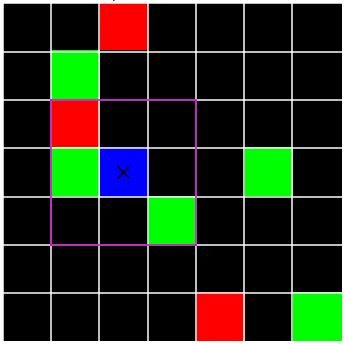
\includegraphics[width=0.9\linewidth]{imgs/myopic.png}
			\caption{\textbf{The myopic agent} only sees a $3\times3$ window centered at its position.}
			\label{myopic}
		\end{subfigure}
		\begin{subfigure}[b]{.45\linewidth}
			\centering
			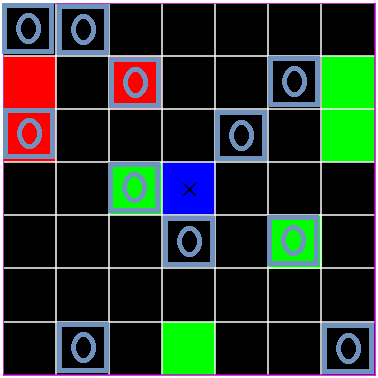
\includegraphics[width=0.9\linewidth]{imgs/masked.png}
			\caption{\textbf{The masked agent} has a receptive field which covers the entire ``noisy'' grid (dropout).}
			\label{masked}
		\end{subfigure}
		\caption{Our GridWorld environment.}
		\label{grid}
	\end{figure}
	
	
	\begin{figure}[!t]
		\centering
		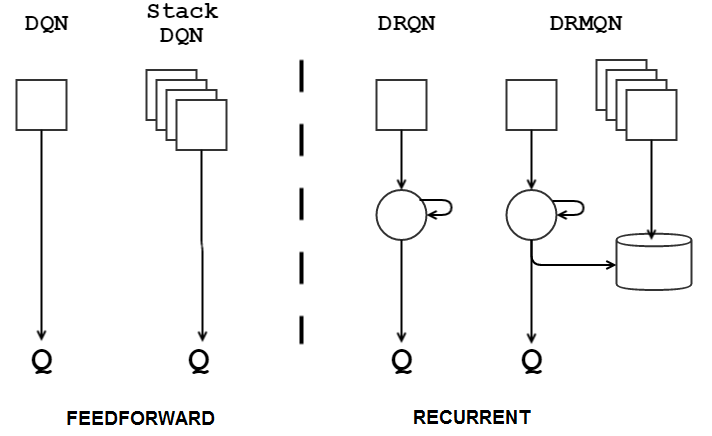
\includegraphics[width=0.75\textwidth]{imgs/schema_archi.png}
		\caption{The 4 types of architecture considered in our work.}
		\label{archi}
	\end{figure}
	
	\paragraph{Considered architectures}: In the following experiments, we consider 4 types of deep net architectures:
	
	\begin{itemize}
		\item \textbf{DQN}: This agent is a feedforward net which only sees one frame at a time.
		\vspace{0.3cm}
		
		\item \textbf{Stack DQN}: This agent is a feedforward net which sees a stack of the $S$ last frames at each timesteps. We always used $S=10$ in our experiments. Note that the high cost of stacking input frames might be prohibitive when the state representation is highly dimensional. 
		\vspace{0.3cm}
		
		\item \textbf{DRQN}: Here, the agent is a recurrent net using LSTM layers. This neural net only sees one state at a time, making it more data-efficient than the Stack DQN approach.
		\vspace{0.3cm}
		
		\item \textbf{DRMQN}: The last architecture is more complex as it has two inputs : one input is the current state and is fed to a recurrent layer; the other input is the stack of the $S$ last frames and is fed to a memory module. This kind of architecture is called Memory Networks [6]. We could say that this architecture is in-between the DRQN agent and the Stack DQN one. The main difference with these architectures is the presence of a memory module coupled with a soft attention mechanism which allows the agent to select among the $S$ frames of the second input which ones are important to look at in priority. This kind of network has been successfully used in [4]: in this work, the memory net architecture obtains the best performance.
		\vspace{0.3cm}
	\end{itemize}
	
	Each of these architectures is represented in Figure \ref{archi}. 
	%More details about the exact architecture (i.e. number of layers, number of neurons, non-linearities...) can be found in the appendix.
	
	\subsection{The myopic agent}
	
	As illustrated in Figure \ref{myopic}, our first experiment corresponds to the following situation: the agent only sees a $3\times3$ block of pixels centered at its position. The task is clearly a POMDP as the state is often ``empty'' (or at least without green cells): in this case, the agent would have to explore unvisited part of the grid in order to discover unseen green cells. Learning curves (i.e. smoothed returns versus the number of completed episodes) are shown in Figure \ref{myopic_curves}. As you can see, the basic DQN agent does not perform well in comparison with other approaches. As in [4], the memory net obtains the best performance. Nervertheless, note that this approach is slightly more costly (see Training time section in the appendix) than other ones and requires an environment in which stacking states is possible. If one has to deal with a very highly dimensional representation space, it would probably be better to adopt the DRQN architecture as this agent only sees one state at a time and clearly outperforms the basic DQN approach. Note that the red curve which is above all other ones is just here as an indication: for this experiment, we allow the agent to see the entire world (i.e. we fall back in the context of a MDP). Therefore, as a conclusion, we observe that, even if it does not permit to obtain the results obtained in the fully observable scenario, adding recurrent layers helps. 
	
	\begin{figure}
		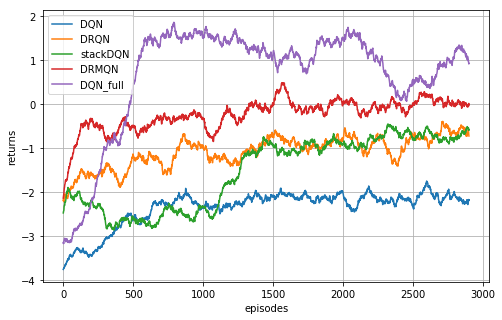
\includegraphics[width=0.75\textwidth]{imgs/myopic_curves.png}
		\caption{Learning curves for the myopic agent experiments.}
		\label{myopic_curves}
	\end{figure}
	
	\subsection{The masked agent}
	
	In our second experiment, partial observability appears in the form of a dropout mask: at each time step, some pixels are uniformly picked and zeroed. The dropout rate is noted $P$. For instance, $P=0.25$ means that at each timestep, $25\%$ of the current state is invisible to the agent (i.e. $25\%$ of the current pixel values are set equal to $0$). Learning curves for different dropout rates are showed in Figure \ref{masked_curves}. As you can see, once again, adding recurrent layers (orange curve) helps. However, in this experiment, the DRMQN approach does not good results, which is a bit disappointing as it was the best architecture in our first experiment. On the contrary, the stack DQN approach clearly outperforms other approaches when the dropout rate is high ($P=0.75$). We don't have any good explanation to justify the discrepancy between the stack DQN approach and the memory net one: we expected the latter to work better or at least similarly to the former...
	
	\begin{figure}
		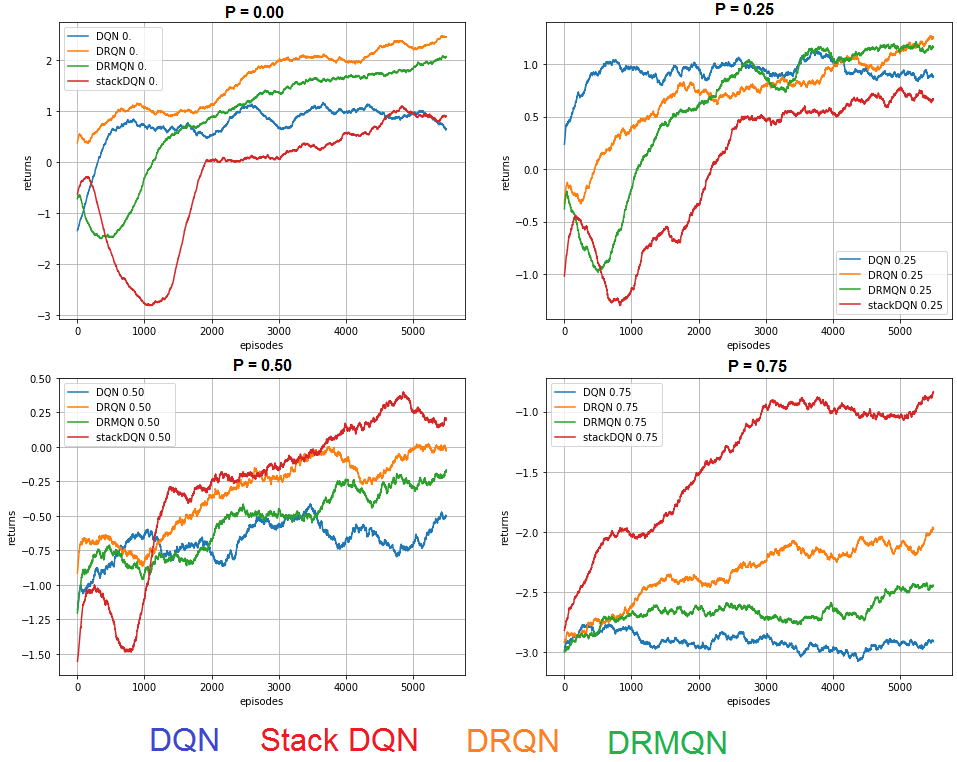
\includegraphics[width=0.95\textwidth]{imgs/masked_curves.png}
		\caption{Learning curves for the myopic agent experiments with different dropout rate values.}
		\label{masked_curves}
	\end{figure}
	
	\subsection{Robustness to Partial Observability}
	
	Finally, we performed one last experiment aimed at evaluating robustness to partial observability at testing time. To do so, we adopted the following strategy:
	
	\begin{itemize}
		\item Train the deep net \textbf{without} partial observability: $P=0$. 
		\item Once the training is completed, evaluate the agent performance with $P=0.5$.
	\end{itemize}
	
	Average cumulative reward (averaged over $500$ episodes) obtained in this context with each architecture is showed in Table \ref{my-label}. Results match our previous conclusion: the stack DQN and the DRQN agent are the best on this POMDP.
	
	\begin{table}[!t]
		\centering
		\caption{Average return for each architecture}
		\label{my-label}
		\begin{tabular}{|c|c|c|c|}
			\hline
			DQN & Stack DQN & DRQN        & DRMQN       \\ \hline
			-2.05  & -1.27  & -1.31 & -1.45 \\ \hline
		\end{tabular}
	\end{table}
	
	\section{Conclusion}
	
	Our experiments suggest that, if one needs to deal with partial observability, stacking states might perform the best. If the state representation is too highly dimensional, the stacking option might be too costly: in that case, recurrent nets would probably the way to go as this kind of architecture is both data-efficient and more robust to partial observability than basic DQN architectures.
	
	\newpage
	
	\setcounter{secnumdepth}{0} %% no numbering
	\section{References}
	\setcounter{secnumdepth}{1} %% Start numbering again
		
	[1]  \textbf{Deep Recurrent Q-Learning for Partially Observable MDPs}, Matthew Hausknecht and Peter Stone, (2015) 
	\vspace{0.1cm}
	
	[2]  \textbf{Playing Atari with Deep Reinforcement Learning}, Volodymyr Mnih, Koray Kavukcuoglu, David Silver, Alex Graves, Ioannis Antonoglou, Daan Wierstra, Martin Riedmiller (2015)
	\vspace{0.1cm}
	
	[3]  \textbf{Asynchronous Methods for Deep Reinforcement Learning} , Volodymyr Mnih, Adrià Puigdomènech Badia1, Mehdi Mirza1, Alex Graves, Tim Harley, Timothy P., David Silver, Koray Kavukcuoglu (2016)
	\vspace{0.1cm}
	
	[4]  \textbf{Control of Memory, Active Perception, and Action in Minecraft} , Junhyuk Oh, Valliappa Chockalingam, Satinder Singh, Honglak Lee (2016)
	\vspace{0.1cm}
	
	[5]  \textbf{Neural Episodic Control} , Alexander Pritzel, Benigno Uria, Sriram Srinivasan, Adria Puigdom, Oriol Vinyals, Demis Hassabis, Daan Wierstra, Charles Blundell (2017)
	\vspace{0.1cm}
	
	[6] \textbf{ End-To-End Memory Networks} , Sainbayar Sukhbaatar, Arthur Szlam, Jason Weston, Rob Fergus (2015)
	\vspace{0.1cm}
	
	[7]   \textbf{Sparse Distributed Memories for On-Line Value-Based Reinforcement Learning} , Bohdana Ratitch, Doina Precup (2004)
	\vspace{0.1cm}
	
	[8]  \textbf{Partial Observability and Deep Recurrent Q-Networks}, Arthur Juliani, (2016) \\Ó https://medium.com/emergent-future/simple-reinforcement-learning-with-tensorflow-part-6-partial-observability-and-deep-recurrent-q-68463e9aeefc
	
	\renewcommand\appendixname{Appendix}
	\renewcommand\appendixpagename{Appendix}
	
	\appendix
	\appendixpage
	
	\section{Training time}
	
	The table \ref{time} shows how long it takes to complete one episode during training for each algorithm:
	
	\begin{table}[!h]
		\centering
		\caption{Time (in seconds) required to complete one episode during training for each architecture.}
		\label{time}
		\begin{tabular}{c|c|c|c|c|}
			\cline{2-5}
			& \textbf{DQN} & \textbf{Stack DQN} & \textbf{DRQN} & \textbf{DRMQN} \\ \hline
			\multicolumn{1}{|c|}{\textit{\textbf{Episode time (s)}}}  & 2.5 s           & 2.8 s              &  2.9 s        & 3.4 s             \\ \hline
		\end{tabular}
	\end{table}
	
	
	As you can see, the simple feedforward DQN is slightly faster than other architectures. A full training on the myopic experiment takes around 2 hours. On the second experiment, it takes around 4 hours.
	
\end{document}



